%%%%%%%%%%%%%%%%%%%%%%%%%%%%%%%%%%%%%%%%%%%%%%%%%%%%%
%                                                   %
%     Penn State Colloquium Poster Template         %
%                                                   %
% Uses Penn State Colloquium class, with options:   %
%                                                   %
% Orientation:                                      %
%     portrait (default), landscape                 %
%                                                   %
% Paper size:                                       %
%     a4paper (default), a0paper, a1paper, a2paper, %
%     a3paper, a5paper, a6paper                     %
%%%%%%%%%%%%%%%%%%%%%%%%%%%%%%%%%%%%%%%%%%%%%%%%%%%%%
\documentclass{../psuposter}
\renewcommand{\templateimagepath}{../} 


%%%%%%%%%%%%%%%%%%%%%%%%%%%%%%%%%%%%%%%%%%%%%%%%%%%%%
%               Package Dependencies                %
%%%%%%%%%%%%%%%%%%%%%%%%%%%%%%%%%%%%%%%%%%%%%%%%%%%%%
\usepackage{natbib}
\usepackage{lipsum}                                % Dummy text
\usepackage[figwidth = 0.98\linewidth]{todonotes}  % Dummy image (and more!)
\usepackage[absolute, overlay]{textpos}            % Figure placement
\usepackage{braket}
\setlength{\TPHorizModule}{\paperwidth}
\setlength{\TPVertModule}{\paperheight}
\setcitestyle{numbers,square}


%%%%%%%%%%%%%%%%%%%%%%%%%%%%%%%%%%%%%%%%%%%%%%%%%%%%%
%                 AUTHOR AND TITLE                  %
%%%%%%%%%%%%%%%%%%%%%%%%%%%%%%%%%%%%%%%%%%%%%%%%%%%%%
\title{The Magic of Moiré Quantum Matter}
\author{Pablo Jarillo-Herrero}
\institute{Massachusetts Institute of Technology}


%%%%%%%%%%%%%%%%%%%%%%%%%%%%%%%%%%%%%%%%%%%%%%%%%%%%%
%                  BEGIN DOCUMENT                   %
%%%%%%%%%%%%%%%%%%%%%%%%%%%%%%%%%%%%%%%%%%%%%%%%%%%%%
\begin{document}
\begin{frame}
\begin{columns}[t, totalwidth=\textwidth]
\begin{column}{0.45\textwidth - 1cm}


%%%%%%%%%%%%%%%%%%%%%%%%%%%%%%%%%%%%%%%%%%%%%%%%%%%%%
%                 BLOCK: BIOGRAPHY                  %
%%%%%%%%%%%%%%%%%%%%%%%%%%%%%%%%%%%%%%%%%%%%%%%%%%%%%
    \begin{block}{Speaker Biographic Summary}
    	\begin{center}
    		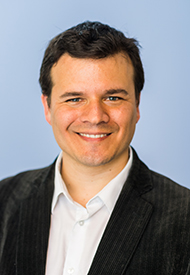
\includegraphics[width=0.45\textwidth]{images/portrait}
    	\end{center}
    	\href{http://jarilloherrero.mit.edu}{Dr. Pablo Jarillo-Herrero} is currently the Cecil and Ida Green Professor of Physics at MIT. 
    	After receiving his Ph.D. from Delft University in 2005, he moved to Columbia University, where he worked as a NanoResearch Initiative Fellow, then joined the MIT faculty 2008.
    	His awards include the Spanish Royal Society Young Investigator Award (2006), an NSF Career Award (2008), an Alfred P. Sloan Fellowship (2009), a David and Lucile Packard Fellowship (2009), the IUPAP Young Scientist Prize in Semiconductor Physics (2010), a DOE Early Career Award (2011), a Presidential Early Career Award for Scientists and Engineers (PECASE, 2012), an ONR Young Investigator Award (2013), Moore Foundation Experimental Physics in Quantum Systems Investigator Award (2014), APS Oliver E. Buckley Prize (2020), and the Wolf Prize in Physics (2020). 
%    	Prof. Jarillo-Herrero has been selected as a Highly Cited Researcher by Clarivate Analytics-Web of Science (2017-2019), and was elected APS Fellow (2018), Fellow of the Quantum Materials Program of the Canadian Institute for Advanced Research (CIFAR, 2019), and Member at Large of the APS Division of Condensed Matter Physics (2019).
    \end{block}


%%%%%%%%%%%%%%%%%%%%%%%%%%%%%%%%%%%%%%%%%%%%%%%%%%%%%
%            BLOCK: RESEARCH INTERESTS              %
%%%%%%%%%%%%%%%%%%%%%%%%%%%%%%%%%%%%%%%%%%%%%%%%%%%%%
    \begin{block}{Research Interests}
        Professor Jarillo-Herrero's research interests lie in the area of experimental condensed matter physics, in particular quantum electronic transport and optoelectronics in novel two-dimensional materials such as graphene and topological insulators, with special emphasis on investigating their superconducting, magnetic, and topological properties. His group uses both transport and optical methods to probe and manipulate ultrathin magnets with potential applications in spintronics. The group also employs electrostatic doping to electrically control the magnetic ground state of these materials.

        \begin{center}
	    	
\includegraphics[width=0.65\textwidth]{images/research}\\       
	    	\textit{Magic angle graphene superlattice.} 		
    	\end{center}


    \end{block}
\end{column}
\begin{column}{0.55\textwidth - 1cm}


%%%%%%%%%%%%%%%%%%%%%%%%%%%%%%%%%%%%%%%%%%%%%%%%%%%%%
%                 BLOCK: ABSTRACT                   %
%%%%%%%%%%%%%%%%%%%%%%%%%%%%%%%%%%%%%%%%%%%%%%%%%%%%%
    \begin{block}{Talk Abstract}
    	Moiré superlattices have recently emerged as a novel platform where correlated physics and superconductivity can be studied with unprecedented tunability. Although correlated effects have been observed in several other moiré systems, magic-angle twisted bilayer graphene (MATBG) remains the only one where robust superconductivity has been reproducibly measured. In this talk I will present a new moiré superconductor, mirror symmetric magic-angle twisted trilayer graphene (MATTG) with dramatically richer tunability in electronic structure and superconducting properties. Hall effect and quantum oscillations measurements as a function of density and electric field allow us to determine the system's tunable phase boundaries in the normal state. Zero magnetic field resistivity measurements then reveal that the existence of superconductivity is intimately connected to the broken symmetry phase emerging at two carriers per moiré unit cell. Strikingly, we find that the superconducting phase gets suppressed and bounded at the van Hove singularities (vHs) partially surrounding the broken-symmetry phase, which is difficult to reconcile with weak-coupling BCS theory. Moreover, the extensive in situ tunability of our system allows us to achieve the ultra-strong coupling regime, characterized by a Ginzburg-Landau coherence length reaching the average inter-particle distance and very large $T_BKT/T_F$ ratios in excess of 0.1. These observations suggest that MATTG can be electrically tuned close to the two-dimensional BCS-BEC crossover. Our results establish a new generation of tunable moiré superconductors with the potential to revolutionize our fundamental understanding and the applications of strong coupling superconductivity.
    \end{block}


%%%%%%%%%%%%%%%%%%%%%%%%%%%%%%%%%%%%%%%%%%%%%%%%%%%%%
%                BLOCK: BACKGROUND                  %
%%%%%%%%%%%%%%%%%%%%%%%%%%%%%%%%%%%%%%%%%%%%%%%%%%%%%
    \begin{block}{Brief Background}
    	Apart from stacking two-dimensional building blocks on top of each other, the properties of Van der Waals heterostructures can be also tuned by introducing a twist angle between different layers. Interestingly, this system exhibits strongly correlated electronic properties, for example the material behaves as a Mott insulator, showing correlated insulating or non-conducting states as a result of their bands being flat near zero Fermi energy. \cite{caoSuperlatticeInducedInsulatingStates2016} \cite{caoUnconventionalSuperconductivityMagicangle2018}

        \begin{center}
		   	
\includegraphics[width=0.65\textwidth]{images/background}    		
    	\end{center}
		Strong spatial suppression in low dimensional materials (LDMs) leads to novel light-matter interactions and allowing for dramatic electrical control and efficient detection of light. \cite{xiaTwodimensionalMaterialNanophotonics2014}  

    \end{block}


%%%%%%%%%%%%%%%%%%%%%%%%%%%%%%%%%%%%%%%%%%%%%%%%%%%%%
%                 BLOCK: REFERENCES                 %
%%%%%%%%%%%%%%%%%%%%%%%%%%%%%%%%%%%%%%%%%%%%%%%%%%%%%
    \begin{block}{References}
        \bibliographystyle{aipnum4-1}
%        \bibliographystyle{iopart-num}
		\bibliography{references}
    \end{block}

\end{column}
\end{columns}


%%%%%%%%%%%%%%%%%%%%%%%%%%%%%%%%%%%%%%%%%%%%%%%%%%%%%
%                    FOOTER TEXT                    %
%%%%%%%%%%%%%%%%%%%%%%%%%%%%%%%%%%%%%%%%%%%%%%%%%%%%%
\begin{textblock}{0.5}(0.18, 0.94)
    \color{white}
    \sffamily
    \textbf{Eberly College of Science}
    \\
    Department of Physics
\end{textblock}


%%%%%%%%%%%%%%%%%%%%%%%%%%%%%%%%%%%%%%%%%%%%%%%%%%%%%
%                   END TEMPLATE                    %
%%%%%%%%%%%%%%%%%%%%%%%%%%%%%%%%%%%%%%%%%%%%%%%%%%%%%
\end{frame}
\end{document}
